\chapter{Technische Grundlagen}
\label{ch:background}
In diesem Kapitel werden alle nötigen technischen Grundlagen zusammengetragen. Da es sich um ein OAuth2 System handelt, wird diese Spezifikation erläutert. Zudem werden auf die Tokens eingegangen, die die Ressource Server jeweils validieren müssen. Diese sind \ac{JSON} Web Token. Dann werden noch die Metriken zum Messen der Performance erläutert, das Programm zum Messen dieser Werte genannt sowie das Framework zur Implementierung der Ressource Server erklärt. 

%
% Section: Der erste Abschnitt
%
\section{Grundlegender Begriffe der IT-Sicherheit}
\label{sec:background:first_section}
Im Bereich der IT-Sicherheit gibt es eine Reihe relevanter Begriffe, die regelmäßig verwendet werden.

\begin{description}
  \item[Authentifizierung:] Bei einer Authentifizierung beweist ein Nutzer seine Identität, indem er dem gegenüberliegenden Server Informationen übermittelt, über die nur der Nutzer verfügen kann wie beispielsweise ein Nutzername und Passwort oder ein Token.
  \item[Autorisierung:] Eine Autorisierung findet grundsätzlich nach der Authentifizierung statt. Hier überprüft das System nach der Authentifizierung des Nutzers, ob der Nutzer über die notwendigen Rechte verfügt eine Aktion auszuführen. 
  \item[Integrität:] Bei der Integrität wird verifiziert, dass Daten seit ihrer Erstellung nicht verändert wurden. Dies kann beispielsweise durch eine Signatur, die nur der Ersteller der Daten erstellen kann, gewährleistet werden [5].
  \item[Authentizität:] Das Ziel der Authentizität ist die Verifizierung des Erstellers der Daten [5]. Das bedeutet, es soll möglich sein zu überprüfen, dass die Daten, die zugesendet werden, auch tatsächlich von der Person oder dem System kommen, von der man annimmt das sie der Urheber ist.
  \item[Validierung] Man kann von einer Validierung sprechen, wenn oben genannte Aspekte, nämlich die Authentifizierung, Autorisierung, Integrität sowie Authentizität, überprüft werden.
\end{description}

%
% Section: Der Zweite Abschnitt
%
\section{OAuth2}
\label{sec:background:second_section}
OAuth2 ist eine Spezifikation, die ursprünglich entwickelt wurde, um Dritten Zugriff auf die Daten eines sogenannten Ressource Owners zu ermöglichen, ohne dass dieser Ressource Owner dem Dritten, in der Spezifikation Client genannt, sein Nutzername und Passwort übermitteln muss [6].  Dies wird dadurch ermöglicht, dass dem Client von einem Autorisationsserver ein Token übermittelt wird und mit diesem Token kann der Client Daten des Ressource Owners abfragen oder Aktionen im Namen des Ressource Owners durchführen. Diese Daten des Ressource Owners werden auf dem sogenannten Ressource Server gehostet.
Im Laufe der Zeit wurde diese Spezifikation erweitert, um weitere Anwendungsfälle abzudecken, wie die Spezifikation OpenID Connect, welche Single-Sign-On ermöglicht. 

\subsection{Rollen in OAuth2}
\label{subsec:background:second_section:first_subsection}
Es gibt vier verschiedene Rollen, die in OAuth2 spezifiziert sind.

\begin{description}
  \item[Ressource Owner:] Der Ressource Owner ist dazu in der Lage, Dritten Zugriff auf seine Daten zu geben oder Aktionen in seinem Namen durchzuführen [7]. Falls der Ressource Owner eine Person ist, nennt man ihn den End-Nutzer.
  \item[Ressource Server:] Der Ressource Server hostet die geschützten Ressourcen des Ressource Owners und ist in der Lage Anfragen zu diesen Ressourcen zu beantworten, falls ein valider Token, ein sogenannter Access Token, in der Anfrage zur Ressource vorliegt [7].
  \item[Client:] Der Client ist diejenige Komponente, die die Ressource des Ressource Owner's von dem Ressource Servers erlangen möchte und dafür einen Access Token benötigt [7]. 
  \item[Authorization Server:] Der Authorization Server verteilt Access Token falls sich der Ressource Owner erfolgreich authentifiziert und gegebenenfalls den Client autorisiert hat, Aktionen durchzuführen. 
\end{description}

\subsection{Erhalt von Token}
\label{subsec:background:second_section:second_subsection}

Gemäß der Spezifikation gibt es fünf verschiedene Wege, wie ein Client von einem Authorization Server einen Token erhalten kann [8]. Im Folgenden werden nur lediglich zwei beschrieben, da die anderen drei für diese Arbeit keine Relevanz haben. 

\subsubsection{Authorization Code Grant}
\label{ssubsec:background:second_section:first_subsection:first_subsubsection}
Bei dem Authorization Code Grant wird der Ressource Owner, der einen Webbrowser verwendet, von dem Client auf den Authorization Server weitergeleitet, um den Ressource Owner zu bitten, sich bei dem Authorization Server zu authentifizieren, um dann dem Client zu autorisieren auf eine geschützte Ressource des Ressource Servers zuzugreifen [9]. 

\subsubsection{User Password Credential Grant}
\label{ssubsec:background:second_section:first_subsection:second_subsubsection}
Diese Art des Token-Erhalts ist ähnlich zu dem Authorization Code Grant, nur dass hier kein Webbrowser notwendig ist, den der End-Nutzer bedient. Stattdessen werden die Authentifizierungsdetails des End-Nutzers, also Nutzername und Passwort, in dem Body der Token-Anfrage übertragen [12]. Im Allgemeinen gilt diese Methode als nicht sicher, allerdings wird sie zu Testzwecken eingesetzt und so auch hier, damit Apache JMeter automatisch einen Token von dem Authorization Server erhalten kann.

\begin{figure}[htbp]
  \centering
  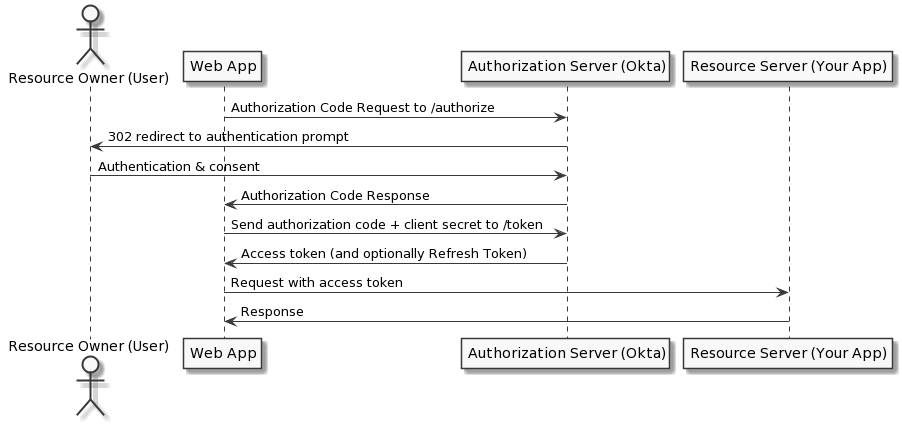
\includegraphics[width=1.0\textwidth]{gfx/oauth_auth_code_flow.png}
  \caption{Dies ist eine einfache Grafik}
  \label{fig:chapter02:Bild1}
 \end{figure}